\documentclass{csmathnotes}

\usepackage{textgreek}

\usepackage{biblatex}

\graphicspath{{images/}}

\udc{519.681}

\title{О задаче различения изображений, состоящих из изолированных пикселей}

\author{Парфёнов Павел Геннадиевич}
\author{Лефанова Дарья Алексеевна}
\author{Лефанов Даниил Сергеевич}
\affiliation{Ярославский государственный университет им. П.\,Г. Демидова}
\email{pavel-parfe@yandex.ru}
\email{zhivaevada@mail.ru} 
\email{daniil.lefanov@yandex.ru}

\addbibresource{bibliography.bib}

\begin{document}

\maketitle

\begin{abstract}	
В настоящей работе применяется подход, использующий характеристический набор коэффициентов изображения для решения двух задач: определение возможности идентичности двух изображений, состоящих из изолированных пикселей; идентификация точки с измененными координатами. Для решения данных задач к указанному подходу были добавлены шаги: соединение точек каждого изображения для решения первой задачи; сравнение характеристических наборов окрестностей точек для решения второй задачи. Данный подход был реализован программно, на рисунках представлены примеры работы программы.

\keywords{цифровое изображение, характеристический набор коэффициентов изображения, эйлерова характеристика}.
\end{abstract}

Цель настоящего исследования заключается в выявлении возможности использования характеристических наборов для определения разницы между двумя изображениями, которые состоят из изолированных пикселей. Задачи исследования состоят, во-первых, в создании алгоритма различения двух изображений, состоящих из изолированных пикселей, с помощью характеристического набора; и, во-вторых, в установлении способа идентификации точки, изменившей своё положение относительно своих изначальных координат.

Отправным пунктом к постановке настоящих задач была задача астроориентации, которая, например, рассмотрена в~\cite{1}. В нашем подходе был опробован характеристический набор коэффициентов чёрно-белого изображения~\cite{4}, который, в отличие от эйлеровой характеристики, описывающей изображение одним числом, описывает изображение как вектор, что позволяет работать с изображением более детально, а также даёт необходимую информацию о топологических и геометрических свойствах изображения~\cite{5}.

\begin{figure}[h!]
	\center{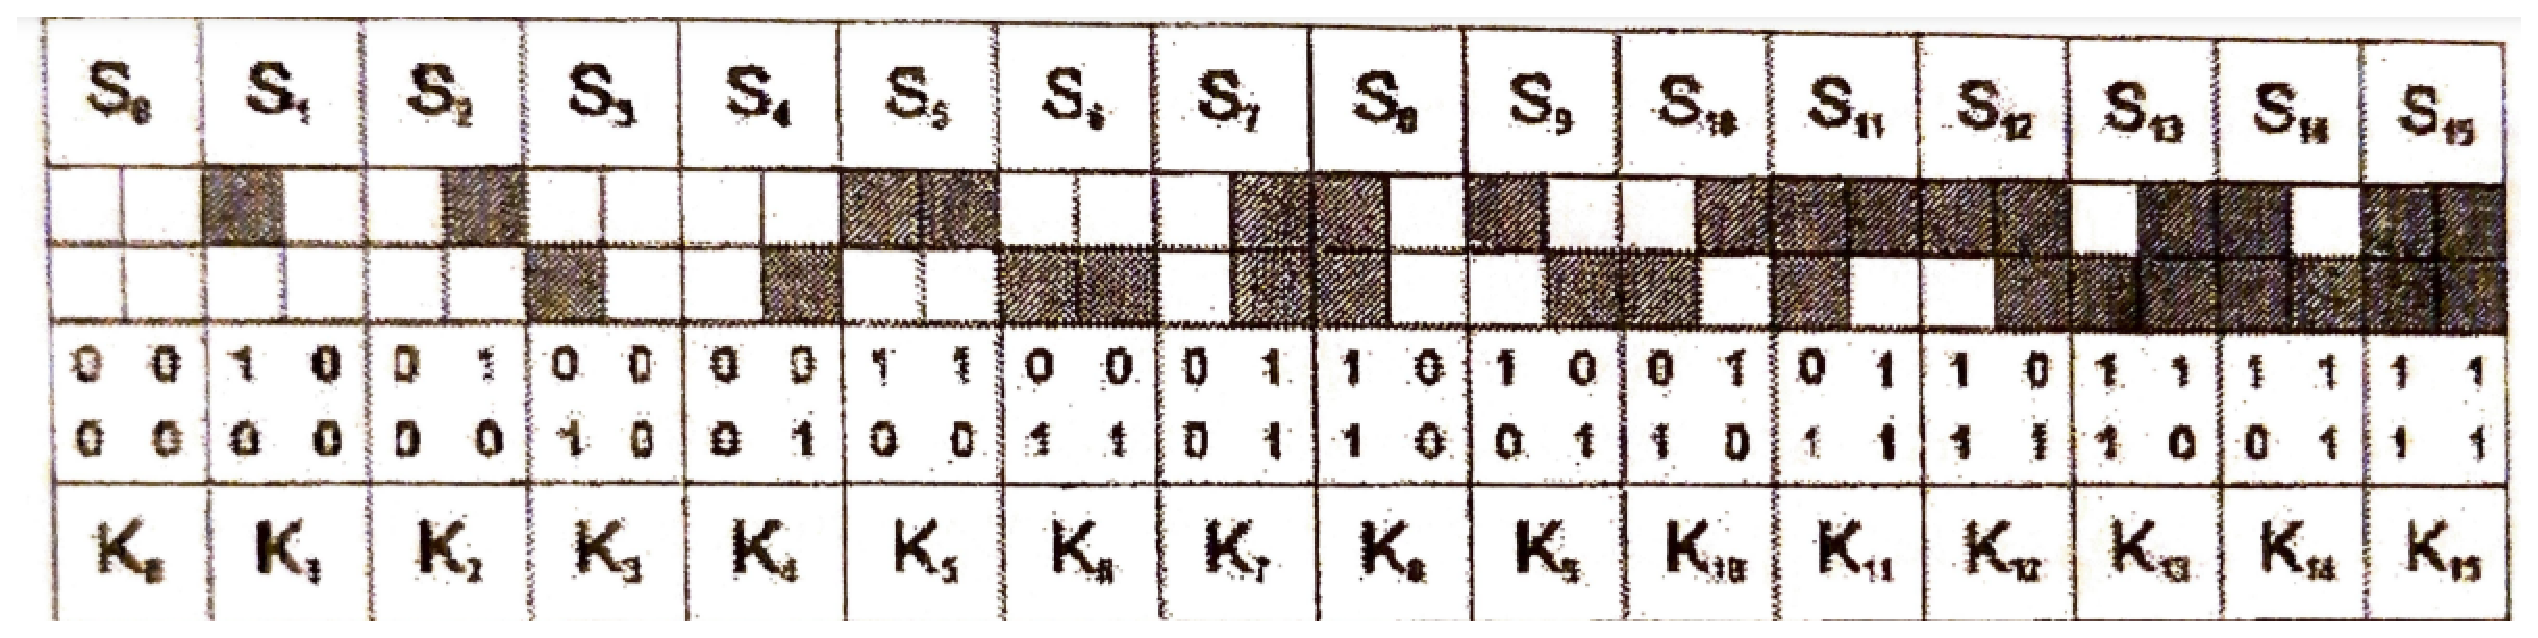
\includegraphics[width=1\linewidth]{image1}}
	\caption{Характеристический набор коэффициентов~\cite{3}.}
	\label{ris1}
\end{figure}

Напомним более детально опеделение характеристического набора~\cite{3}. Выше приведена таблица (см. рис.~\ref{ris1}), в которой показаны 16 коэффициентов изображения, построенных по системе фрагментов размером $2\times2$: во второй строке представлен геометрический аналог соответствующего фрагмента; в третьей строке таблицы указан тип подматрицы, репрезентирующей данный фрагмент. Четвёртая строка — набор неотрицательных целых чисел, указывающих число вхождений фрагментов данного типа в изображение, и этот набор представляет собой шестнадцатимерный вектор, то есть характеристический набор.

Каждое изображение анализируется с позиции количества данных фрагментов; в частности, вычисляется количество фрагментов каждого типа в данном изображении. Следующие выводы построены по результатам сравнения наборов двух изображений.

\begin{figure}[h!]
	\center{\includegraphics[width=1\linewidth]{image2}}
	\caption{Изображения, состоящие из изолированных пикселей.}
	\label{ris2}
\end{figure}

Подобные инструменты ранее были использованы для решения других задач, в частности, для вычисления эйлеровой характеристики и последующей оценки числа связных элементов изображения~\cite{6}, а также для различения элементов отдельных алфавитов~\cite{2}. 

\begin{figure}[h!]
	\center{\includegraphics[width=1\linewidth]{image3}}
	\caption{Характеристический набор для изображений из рис.~\ref{ris2}.}
	\label{ris3}
\end{figure}

Рассмотрим первую задачу, которая состоит в установлении возможности применения характеристического набора для определения идентичности изображений, состоящих из изолированных пикселей.

Необходимо учесть, что, рассчитывая характеристический набор для изображений с одинаковым количеством изолированных пикселей, мы не сможем выявить возможность идентичности изображений, так как их характеристические наборы в любом случае будут одинаковы.

Воспользуемся следующим подходом: соединим все точки отрезками и построим характеристический набор для получившихся изображений (см. рис.~\ref{ris2} и~\ref{ris3}).

На рис.~\ref{ris2} можно увидеть, что характеристические наборы разных изображений отличаются. Характеристические наборы идентичных изображений будут совпадать (см. рис.~\ref{ris4}).

\begin{figure}[h!]
	\center{\includegraphics[width=1\linewidth]{image4}}
	\caption{Пример одинаковых характеристических наборов.}
	\label{ris4}
\end{figure}

Рассмотрим теперь диагностику несовпадений изображений. Возьмём два изображения, отличающихся друг от друга расположением одной (внутренней) точки (см. рис.~\ref{ris5}).

\begin{figure}[h!]
	\center{\includegraphics[width=1\linewidth]{image5}}
	\caption{Сдвиг точки.}
	\label{ris5}
\end{figure}

Как и выше, здесь необходимо соединить точки каждого изображения между собой. Для решения задачи рассмотрим окрестность (подматрицу $7\times7$ пикселей) вокруг каждой изначальной точки и составим характеристический набор для каждой из этих окрестностей, объединив в пары соответствующие друг другу на первом и втором рисунках  (см. рис.~\ref{ris6}).  

\begin{figure}[h!]
	\center{\includegraphics[width=1\linewidth]{image6}}
	\caption{Пример окрестностей пары точек.}
	\label{ris6}
\end{figure}

Пример характеристических наборов для пары соответствующих точек представлен в виде таблицы и графика на рис.~\ref{ris7}:

\begin{figure}[h!]
	\center{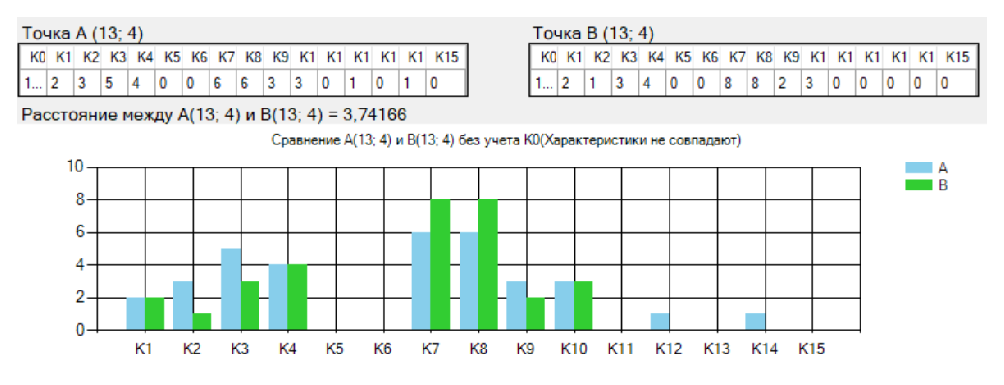
\includegraphics[width=1\linewidth]{image7}}
	\caption{Сравнение характеристических наборов пары откестностей.}
	\label{ris7}
\end{figure}

Далее рассчитывается евклидово расстояние между характеристическими наборами (шестнадцатимерными векторами) соответствующих окрестностей каждой пары точек, то есть между вектором, описывающим окрестность первой точки (начальное положение  точки, изображение А (слева), см. рис.~\ref{ris6}) и вектором, описывающим окрестность второй точки (конечное положение  точки, изображение В (справа), см. рис.~\ref{ris6}). Та пара окрестностей, которая обнаруживает наибольшее расстояние относительно расстояний в других парах, содержит точки с разными координатами.

В ходе работы было доказано, что описанный выше подход с использованием характеристического набора коэффициентов изображения применим к решению задачи различения изображений, состоящих из изолированных пикселей, а также к задаче идентификации точки, изменившей свое положение относительно начальных координат. Данный подход был программно реализован, результат программы показан на рисунках.

\printbibliography

\end{document}
